\section{Complete Coding Examples}
In this section we show coding examples to demonstrate to the reader how to set up a complete model. As we move on, we'll gradually add more customization options to our model setup to have more flexibility. We'll also show how to save and plot data obtained from our simulation, e.g. the pedestrians attributes such as positions and velocity, and also model attributes such as the Hamiltonian. The only files that we will be using from the root project directory are:
\begin{itemize}
    \item \texttt{/activate\_package.jl}
    \item \texttt{/PH\_Project/src/module\_ph\_ped.jl}
\end{itemize}
As we will see in our example, the very first step to start a project would always be to activate the package by executing \texttt{activate\_package.jl}. For any advanced customization, for e.g. changing the numerical solver for the \texttt{stochastic\_ode\_step}, we will have to manually modify the function \autoref{code:sde_solve} within the \texttt{module\_ph\_ped.jl}.

\subsection{Model Setup}
To begin with our examples, let us create a new julia file \texttt{/main.jl} and activate our package.

\begin{listing}[H]
\begin{minted}[escapeinside=??,frame=single, fontsize=\small]{julia}
include("./activate_package/activate_package.jl")
\end{minted}
\end{listing}

\subsubsection*{Example 1: Minimal model setup with default parameter values}
\begin{listing}[H]
\begin{minted}[escapeinside=??,frame=single, fontsize=\small]{julia}
model = initialize()
\end{minted}
\caption{Minimal code to construct a model with default parameter values}
\label{code:ex1}
\end{listing}
With a simple command shown above \autoref{code:ex1}, we can easily construct and initialize the model with default values. We've initialized the model with 32 pedestrians, in the space of 11 units and 5 units in the x and y directions respectively. To retrieve model properties, for e.g. \texttt{λ}, we can write \texttt{model.λ}. Similarly, for agent properties, we can write \texttt{model[1].pos} to retrieve the position of the agent with index 1.
\begin{listing}[H]
\begin{minted}[escapeinside=@@,frame=single, fontsize=\small]{shell-session}
StandardABM with 32 agents of type Pedestrian
agents container: Vector
space: periodic continuous space with [11.0, 5.0] extent and spacing=0.25
scheduler: fastest
properties: no_disp_H, A, λ, B, dH, dt, sigma, alignment, stoch_dH, 
hamiltonian    
\end{minted}
\caption{Output of \autoref{code:ex1} in the terminal, showing model initialization with default values.}
\label{code:repl_ex1}
\end{listing}

\subsubsection*{Example 2: Model setup with user-defined parameter values}
\label{section:ex2}

\begin{listing}[H]
\begin{minted}[escapeinside=@@,frame=single, fontsize=\small]{julia}
seed = 42
properties = Dict(
    # constants
    :λ => 2, :A => 5, :B => 0.3, :dt => 0.01, :sigma => 0.1,
    # hamiltonian and alignment
    :no_disp_H => 0.0, :hamiltonian => 0.0, :dH => 0.0, :stoch_dH => 0.0,
    :alignment => 0.0
)
number_of_peds = 0
x_len, y_len = 11, 5
num_solver = leapfrog_step
\end{minted}
\caption{Initializing model parameters}
\label{code:ex2}
\end{listing}

If we wish to have flexibility in initializing the model parameters beforehand, we can do that by simply writing the arguments as shown in \autoref{code:ex2} for the \texttt{initialize} function \autoref{code:ex2-1}.
\begin{listing}[H]
\begin{minted}[escapeinside=@@,frame=single, fontsize=\small]{julia}
model = initialize(
    number_of_peds, x_len, y_len, num_solver, properties; seed
    )
\end{minted}
\caption{Initialization of the model with modified parameters from \autoref{code:ex2}}
\label{code:ex2-1}
\end{listing}
As we have created the model with zero pedestrians, we can now manually add the pedestrians into our model space using \texttt{addagent!()} as shown below \autoref{code:ex2-2}, and initialize their attributes.

\begin{listing}[H]
\begin{minted}[escapeinside=@@,frame=single, fontsize=\small]{julia}
rng = Distributions.Xoshiro(seed)
number_of_peds = 40
for i in 1:number_of_peds
    Agents.add_agent!(model;
        pos = [rand(rng)*x_len, rand(rng)*y_len],  # Initial position
        vel = [0.0 ,0.0], # Initial velocity
        u@\sub{i}@ = mod(i,2) == 0 ? [1,0] : [-1,0] # counter_flow
        # u@\sub{i}@ = mod(i,2) == 0 ? [0,1] : [1,0] # cross
        # u@\sub{i}@ = [1.0,0.0] # uni-directional flow
    )
end
\end{minted}
\caption{Initialization of the pedestrians}
\label{code:ex2-2}
\end{listing}

The \texttt{addagent!()} function adds a \texttt{Pedestrian} object as an agent into our model. The attributes of \texttt{Pedestrian} were defined in \autoref{code:agent_def}, and hence \texttt{vel}, \texttt{pos}, and \texttt{u\sub{i}} are initialized in \autoref{code:ex2-2}.
    
\subsection{Running the Model}
Once we are satisfied with our model, the next step is to run it! Naturally, we would also want to keep track of how the model and agent attributes change as the simulation runs. Continuing with the model defined in Example 2, we'll run this model for 100 seconds of simulation time, and save the values of each attribute in the \texttt{adf} and \texttt{mdf} dataframes.

\begin{listing}[H]
\begin{minted}[escapeinside=@@,frame=single, fontsize=\small]{julia}
T = 100
total_steps = T/model.dt # or T/properties[:dt]
mdata = [:hamiltonian, :dH, :no_disp_H, :alignment, :stoch_dH]
adata = [:pos, :vel]
adf, mdf = Agents.run!(model, T; mdata, adata)
\end{minted}
\caption{Running the model and tracking the attributes}
\label{code:ex2-run}
\end{listing}

Here, \texttt{mdf} is a dataframe containing a record of the changes over time of all model attributes declared in \texttt{mdata}, similarly the agents attributes declared in \texttt{adata} are saved in the \texttt{adf} dataframe.

\subsubsection*{Visualizing Model Data}
Once the simulation is finished and the dataframes are obtained, we can easily analyze them. As an example, we will illustrate how we can plot the data, and finally show how we can construct a simple interactive application to simulate our model.

Continuing with the dataframes obtained in \autoref{code:ex2-run}, we will plot them using the \texttt{CairoMakie} backend.
\begin{listing}[H]
\begin{minted}[escapeinside=@@,frame=single, fontsize=\small]{julia}
t = model.dt:model.dt:T
h_data, h_star_data = mdf[2:end,:hamiltonian] , mdf[2:end,:no_disp_H]

CairoMakie.activate!()
fig, ax = lines(t, h_data)
lines!(ax, t, h_star_data, linestyle=:dash, label=L"H^*")

ax.ylabel = "H"
ax.xlabel = "time [s]"
ax.title = "Hamiltonian for counter flow | n = $number_of_peds"
axislegend()
fig
\end{minted}
\caption{Example code to plot model attributes}
\label{code:ex2-mplot}
\end{listing}

Here, we have ignored the data from the first step as it only contains the initialized values of the model. By executing \autoref{code:ex2-mplot}, we'll obtain the following plot \autoref{plot:ex2-mplot}

\begin{figure}[H]
    \centering
    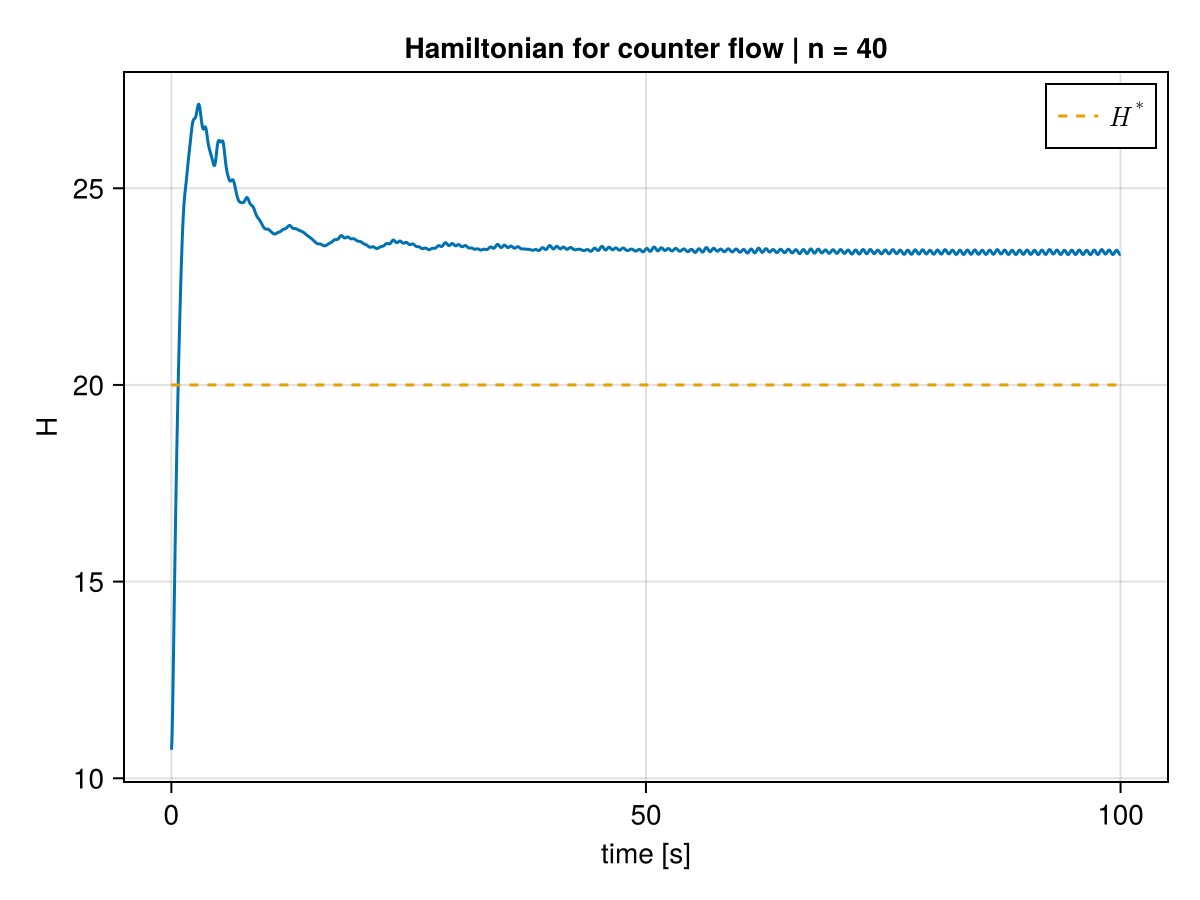
\includegraphics[width=0.5\textwidth]{figures/ch6_tutorial/example_plot.png}
    \caption{Model attribute plot from executing \autoref{code:ex2-mplot}}
    \label{plot:ex2-mplot}
\end{figure}

\subsubsection*{Visualizing Agent Trajectories}
To plot the trajectories of every agent, we use the agent dataframe \texttt{adf} obtained from \autoref{code:ex2-run}. We loop through each \texttt{agent.id} and take its positions within a certain time. Since we have simulated a counter flow \autoref{code:ex2-2}, it would be nice to have a clear distinction between the two groups of agents based on their desired velocities, hence we color them individually.
\begin{listing}[H]
\begin{minted}[escapeinside=@@,frame=single, fontsize=\small]{julia}
path_length = 100
start_time = Int(T/model.dt) - path_length
end_time = start_time + path_length
fig = Figure()
ax = Axis(fig[1, 1], 
          limits = (0,x_len,0,y_len), 
          xlabel = "x_pos", ylabel = "y_pos")
for i in 1:number_of_peds
    if mod(i,2) == 0
        scatter!(ax, adf[adf.id .== i, :].pos[start_time:end_time], 
                color=0:path_length, colormap=:Reds, markersize=5)
    else
        scatter!(ax, adf[adf.id .== i, :].pos[start_time:end_time], 
                color=0:path_length, colormap=:Greens, markersize=5)
    end
end
fig
\end{minted}
\caption{Example code to plot agent trajectories}
\label{code:ex2-aplot}
\end{listing}
We want to see the trajectories of all agents through the 100 timesteps of the simulation. We first set the figure and axis to a defined extent based on the simulation domain that we've defined in \autoref{code:ex2}. Then loop through \texttt{adf}, to get the agent trajectories of each agent. Executing the code results in the plot below

\begin{figure}[H]
    \centering
    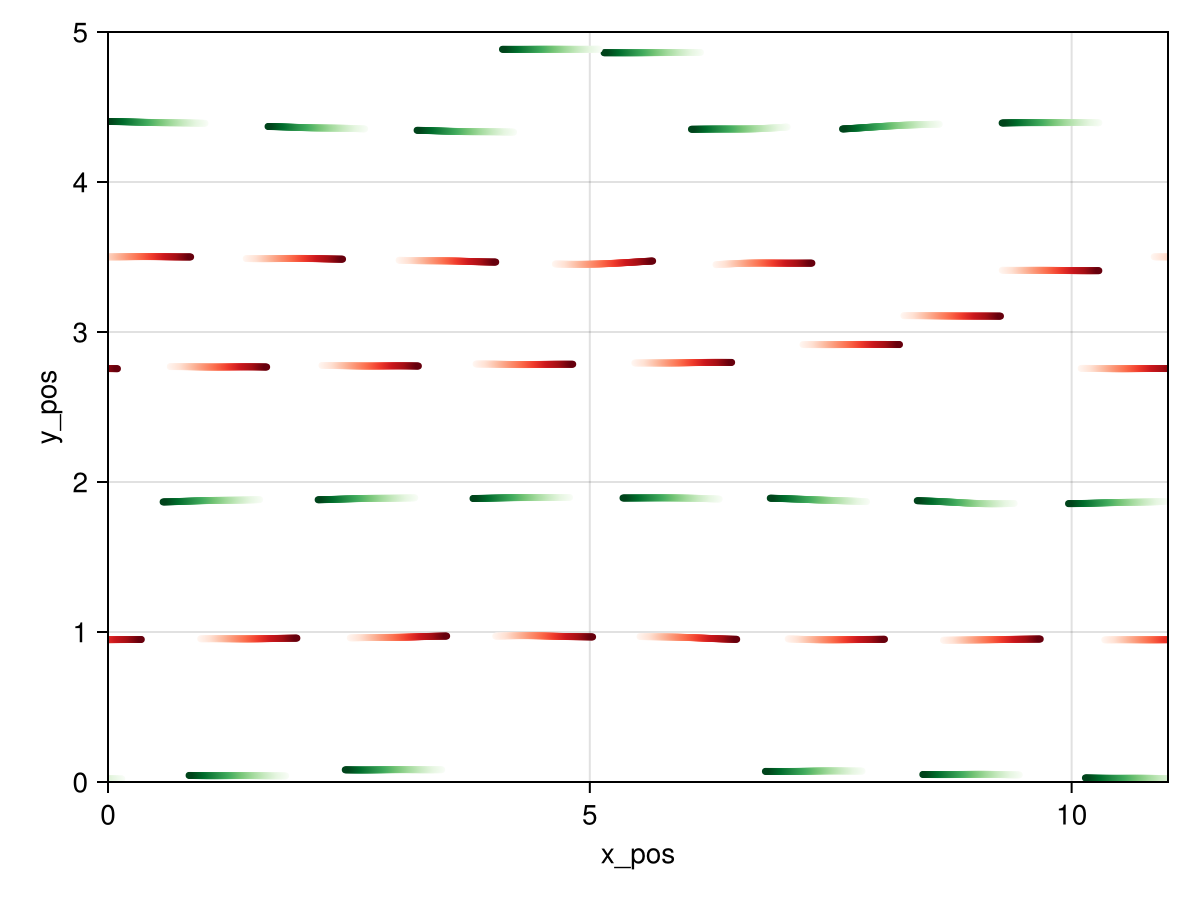
\includegraphics[width=0.5\textwidth]{figures/ch6_tutorial/example_traj.png}
    \caption{Agent trajectories from executing \autoref{code:ex2-aplot}}
    \label{plot:ex2-aplot}
\end{figure}


\subsection{Interactive Visualization}
To construct an interactive application, we'll use the \texttt{GLMakie} backend. Since we want to restart the model every time we open the app, we will initialize the model beforehand, thus we will combine all the codes from example 2 into one function \texttt{model\_init} which will return the initialized model.

To ignore the first initialized values when plotting the data, we run the model for a single time-step using \texttt{Agents.step!(model)}. 
\begin{listing}[H]
\begin{minted}[escapeinside=@@,frame=single, fontsize=\small]{julia}
GLMakie.activate!()
model = model_init()
Agents.step!(model)
params = Dict(
    :λ => 0:0.1:5,
    :A => 0:0.1:10,
    :B => 0:0.1:2,
    :sigma => 0:0.05:1
)
mdata = [:hamiltonian, :dH, :alignment]
fig, abmobs = Agents.abmexploration(model; dt=1:0.2:5, params, mdata)
fig
\end{minted}
\caption{Example code to generate the interactive app}
\label{code:ex2-app}
\end{listing}

Sliders can also be added by creating a dictionary with key value pairs of the model attributes with step ranges shown in \autoref{code:ex2-app}. Finally, to generate the plots of the attributes, we can include \texttt{mdata} with a list of attributes to track, similar to how it was done when running the model in \autoref{code:ex2-run}. With these arguments in \texttt{Agents.abmexploration}, one can create a simple interactive GUI as shown below in \autoref{fig:ex2-app}.

\begin{figure}[H]
    \centering
    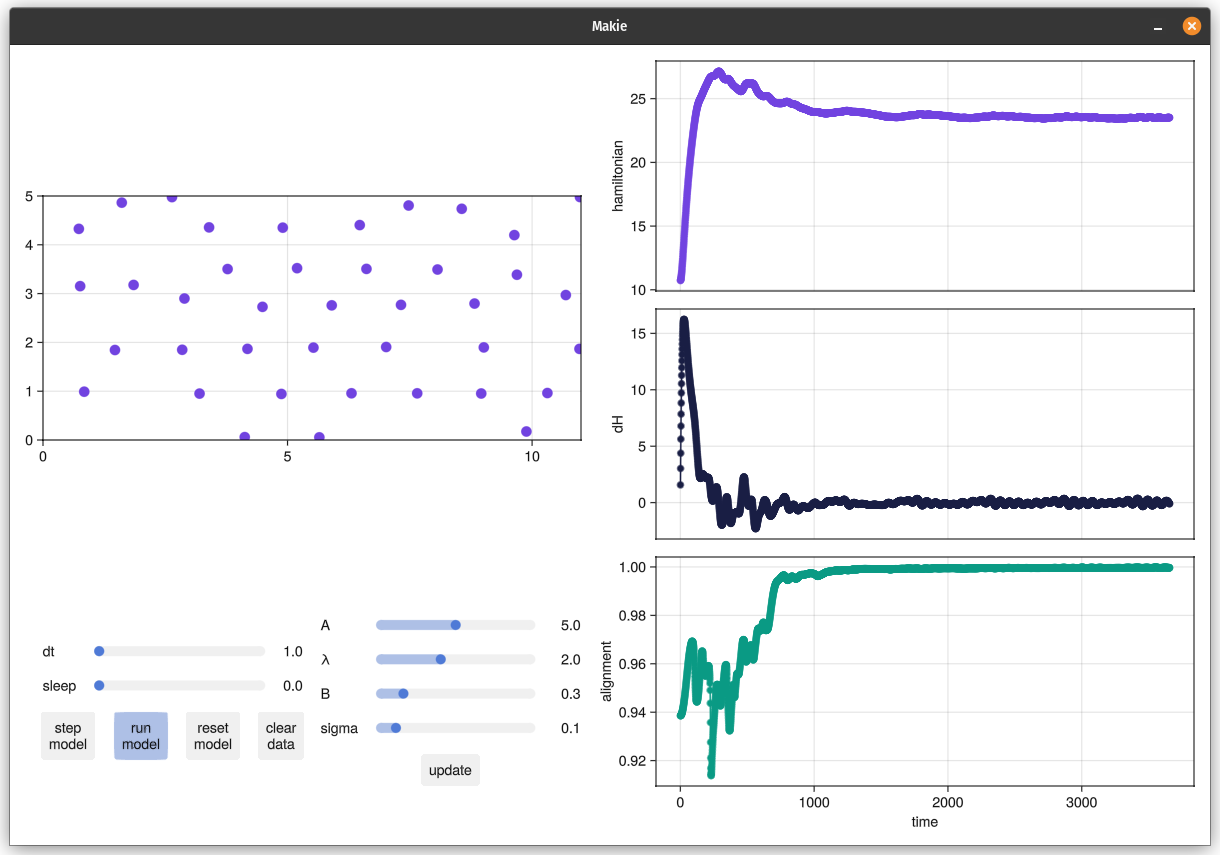
\includegraphics[width=\textwidth]{figures/ch6_tutorial/example_app1.png}
    \caption{Interactive application to simulate the model by executing \autoref{code:ex2-app}}
    \label{fig:ex2-app}
\end{figure}

Of course, with the ease and flexibility provided by the \texttt{Agents.jl} package, one can easily construct more customizable agent based models apps without hassle.

In this section we demonstrated how to easily construct and run our model, we saved and plotted the model and agent data, and finally we also saw how to create an interactive environment to simulate our model with just a few lines of code.